% !TEX root=/home/tavant/these/manuscript/src/manuscript.tex

\section{Axial Convection model}
  \label{sec-reinjectionnoise}
  \inlinenote{Add the section about reinjection noise.}

  As introduce in the previous section, the \ac{2D} radial-azimuthal simulation do not model a priori the convection.

  \subsection{Lafleur's model of injection}

    \citet{lafleur2016a} proposed a way to model the axial convection of the particles in a \ac{1D} purely azimuthal simulation.
    \Cref{fig-Fake_1d_1} shows a schematic illustration of the model.
    The principle is as follow
    \begin{itemize}
      \item We set a finite axial length, noted $L_z$ on \cref{fig-Fake_1d_1}.
      \item We follow the positions of the particle in the axial direction $z$
      \item When a particle crosses the boundary, it is removed.
      \item A new particle is created
      \begin{itemize}
        \item at $z=0$ for the ions
        \item  at $z=L_z$ for the electrons
      \end{itemize}
    \end{itemize}

    We create a new particle in order to conserve the charge in the simulation.
    The new particle has a velocity following a Maxwellian flux distribution function of a given temperature.
    The azimuthal position of the particle is chosen uniformly at random.

    \improvement{Add definition of the Maxellian and maxellian flux VDF ?}

    \begin{figure}[hbtp]
      \centering
      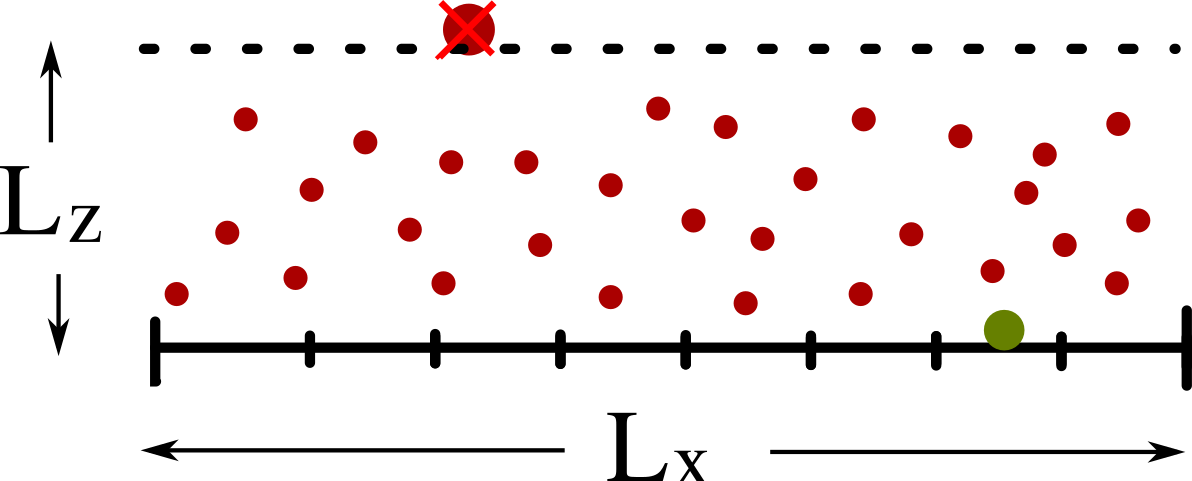
\includegraphics[width=\defaultwidth]{Fake_1d_2}
      \caption{Schematic representation of Trevor's convection model \citep{lafleur2016a}. The red particle is removed of the simulation, and the green particle is created. In this illustration, the particle is an ion. }
      \label{fig-Fake_1d_1}
    \end{figure}

    Lafleur's model of convection has been adopted in \ac{2D} by \citet{croes2017a}.
    The principle is exactly similar.
    The particles are followed in the 3 directions, and a finite length is used to close to axial direction.
    It is important to note that even is the particle are followed in the 3 directions, the meshed domain is only \ac{2D}.
    The simulation is not \ac{3D}-\ac{3V}.

    In \citet{croes2017a}, the authors have observed that if the newly created particle has a radial position chosen uniformly at random, it would affect the sheath.
    Hence, they decided to use the same radial position that the removed particle.
    \Cref{fig-Fake_2d} presents a schematic representation of the convection model in \ac{2D}.

    \begin{figure}[hbtp]
      \centering
      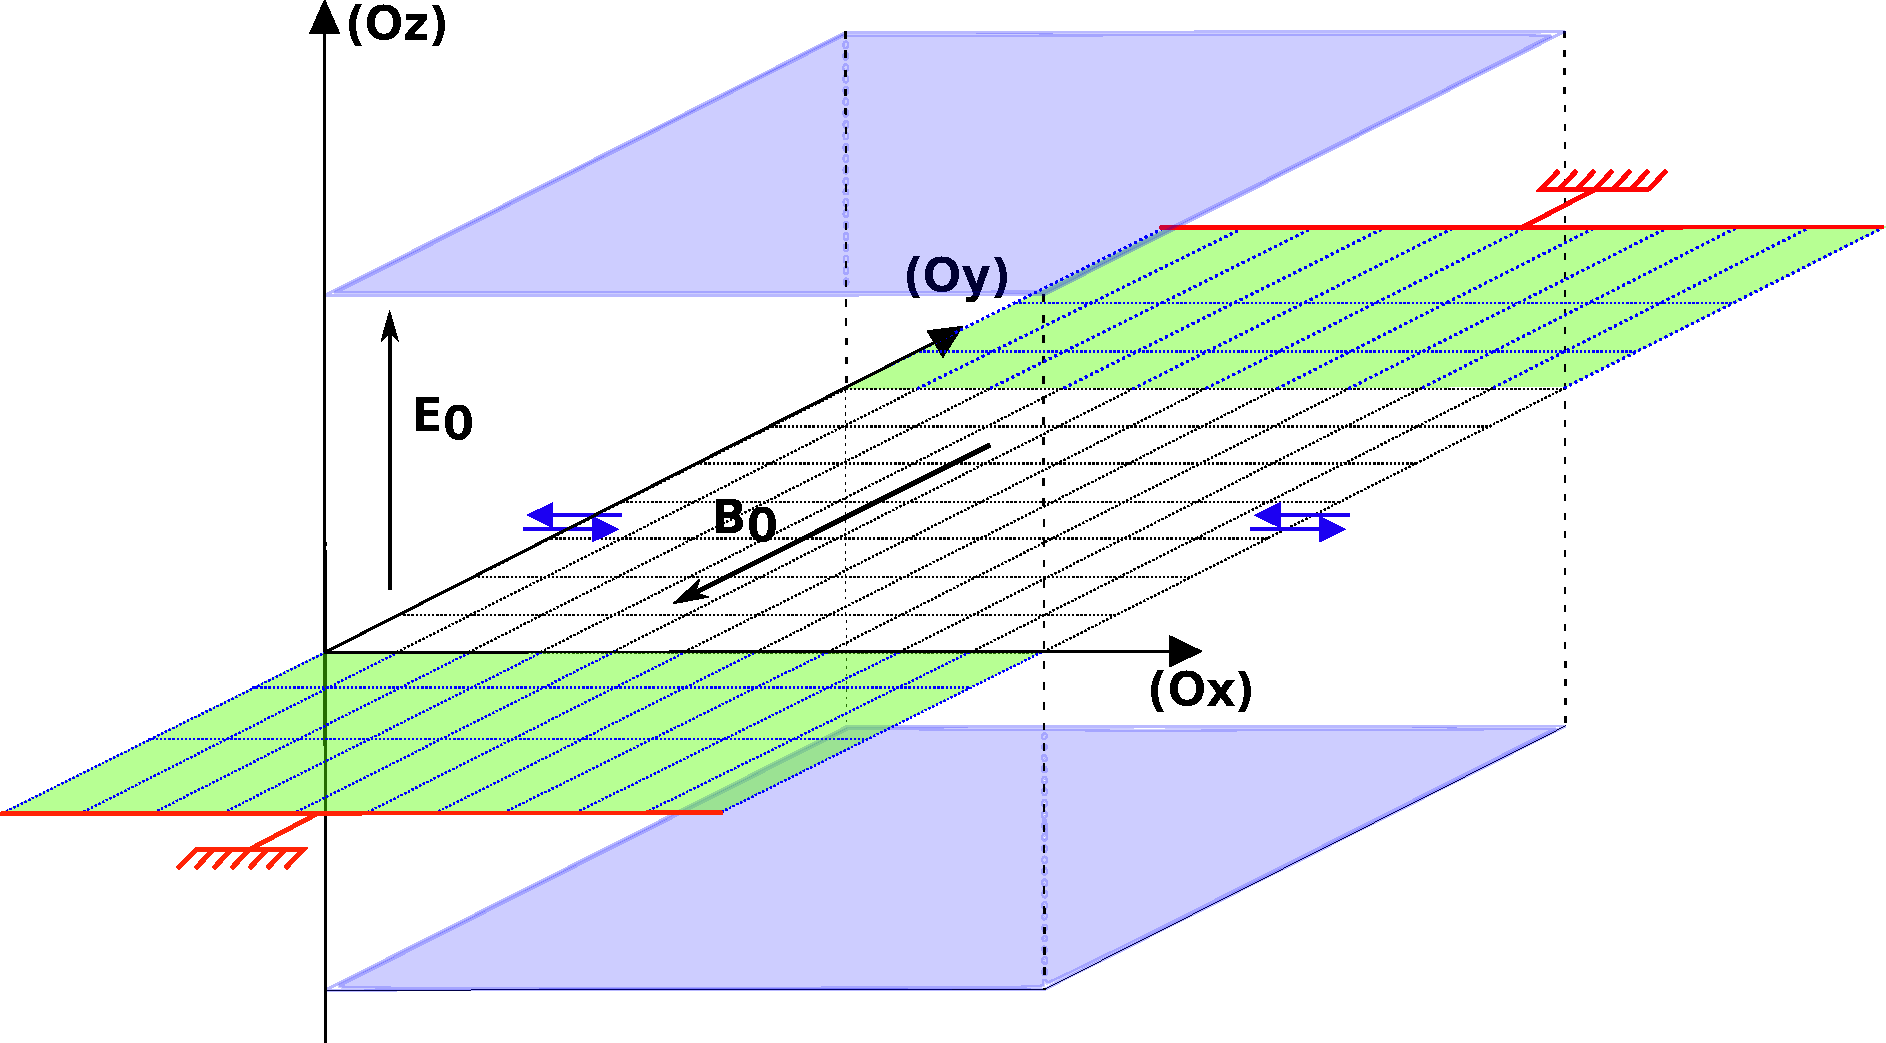
\includegraphics[width=\defaultwidth]{2_5D_dielectric_PPS_small}
      \caption{Schematic representation of the Lafleur's convection model adapted in \ac{2D}. The new particle radial position corresponds to the removed particle, but its azimuthal position is chosen uniformly at random. }
      \label{fig-Fake_2d}
    \end{figure}

    \Cref{fig-energy_convection} shows the evolution as a function of time of the electron mean energy in the simulation in a typical \ac{2D} radial-azimuthal simulation, addapted from \citet{croes2017}.
    We can see that without the convection, the mean energy quickly rises to unphysical values.
    When the convection is modeled, using an axial of $L_z=1$ cm, the energy reaches a steady state.
    \nomenclature[Q]{\ensuremath{ L_z}}{ Axial length}
    \begin{figure}[hbtp]
      \centering
      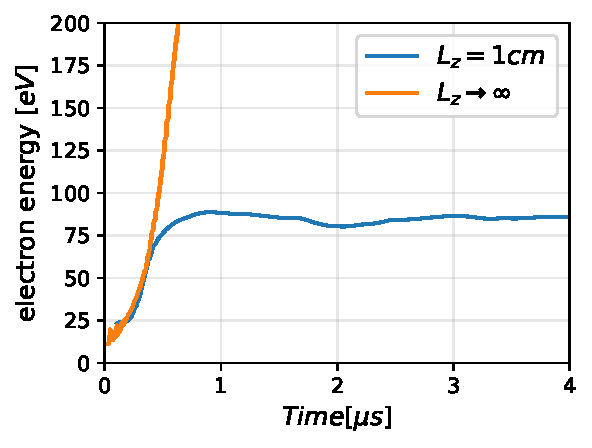
\includegraphics[width=\defaultwidth]{energy}
      \caption{Time evolution of the electron mean energy when the convection is not modeled ($L_z \rightarrow \infty$) and with Trevor's convection model used, $L_z = 1$ cm. Adapted from \citet{croes2017}.}
      \label{fig-energy_convection}
    \end{figure}



  \subsection{Numerical artefacts}
    \citet{lafleur2016a} studied the impact of the convection model on the simulation results.
    The authors observed in particular that changing the azimuthal length of the simulation domain could affect the simulation results.

    \Cref{fig-convection_numerical} shows the time evolution of the azimuthal electric field $E_{\theta}$ from the \ac{1D} simulation \citep{lafleur2016a}.
    \nomenclature[Q]{\ensuremath{ E_{\theta}}}{ Azimuthal electric field}

    On the first row (\cref{fig-convection_numerical}.{\bf a} and {\bf b}), the length of the periodic azimuthal direction is $L_{\theta}=0.5$~cm.
    \cref{fig-convection_numerical}.{\bf a} corresponds to the case without axial convection.
    We clearly see that the \ac{ECDI} rises and do not saturate.
    The wavelength is short, of the order of $\lambda = 1.5$~mm.
    \nomenclature[Q]{\ensuremath{ \lambda}}{ Wave length}
    \cref{fig-convection_numerical}.{\bf b} corresponds to the same case as \cref{fig-convection_numerical}.{\bf a} but this time with the axial convection modeled.
    We observe this time a saturation of the oscillation's amplitude, and the wavelength is close to $\lambda = 1.5$~mm.

    On the second row (\cref{fig-convection_numerical}.{\bf c} and {\bf d}), the length of the periodic azimuthal direction is $L_{\theta}=1$~cm.
    \cref{fig-convection_numerical}.{\bf c} corresponds to the case without axial convection, and \cref{fig-convection_numerical}.{\bf b} corresponds to the same case but this time with the axial convection modeled.
    In \cref{fig-convection_numerical}.{\bf c}, we can see that increasing the azimuthal length did not affect the \ac{ECDI}, as expected.
    However, in  \cref{fig-convection_numerical}.{\bf d}, the instability is clearly affected.
    A simple oscillation is observe, corresponding to $\lambda=10$~mm.
    They are most certainly unphysical.

    \begin{figure}[hbtp]
      \centering

      \begin{tabular}{cc}
        \subfigure{Lafleur_NoLz_1}{a}{20, 20}
            &
        \subfigure{Lafleur_Lz_1}{b}{20, 20} \\

        \subfigure{Lafleur_NoLz_2}{c}{20, 20} &
        \subfigure{Lafleur_Lz_2}{d}{20, 20} \\
      \end{tabular}
      \caption{Effects of Lafleur's convection model for two different azimuthal length on the azimuthal electric field. ({\bf a}) No convection, $L_x=0.5$~cm,  ({\bf b}) convection modeled, $L_x=0.5$~cm,  ({\bf c}) No convection, $L_x=1$~cm,  ({\bf d}) convection modeled, $L_x=1$~cm. The colour of each plots is normalized to the maximum amplitude. Adapted from \citep{lafleur2016a}. \inlinenote{Get $\theta$ back to $y$ instead of $x$}}
      \label{fig-convection_numerical}
    \end{figure}

    \FloatBarrier
    \citet{croes2017} observed similar behaviour with the bidimensional  simulation.
    The author investigated the values of the azimuthal length which presented physical and unphysical results
    for different values of the axial length.
    \Cref{fig-couplesCroes} shows the results obtained (adapted from \citep{croes2017}).
    We can see that for a given value of the axial length, the azimuthal must be lower that a certain value to present physical results.
    However, the value of this upper limit depends of the axial length, such that the if the axial length decreases, the upper limit of the azimuthal length decreases as well.

    \begin{figure}[hbtp]
      \centering
      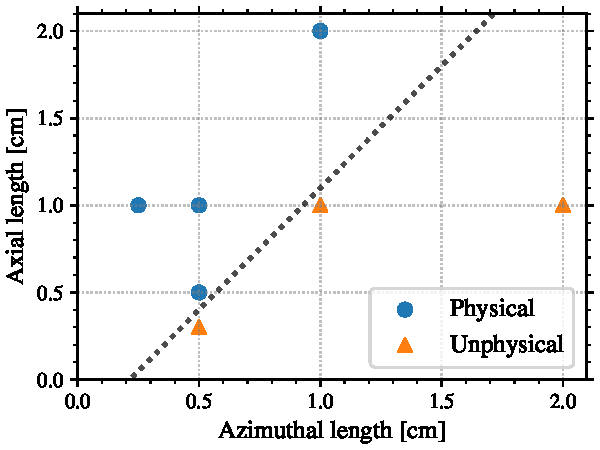
\includegraphics[width=\defaultwidth]{2D_couples}
      \caption{Values of the azimuthal length and the axial length for which the simulation result is physical (similar to \cref{fig-convection_numerical}.{\bf b}) or unphysical  (similar to \cref{fig-convection_numerical}.{\bf d}) \inlinenote{Make this image smaller (smaller font, etc.)}}
      \label{fig-couplesCroes}
    \end{figure}

    No explanation have been proposed, yet.
    In the next section, we develop a possible explanation, and a new convection model for the simulation.

  \subsection{Numerical noise of Lafleur's convection model}

    Let us consider de Lafleur's convection model in \ac{1D} on the charge density.
    When computing the charge density on the mesh vertices, the axial position is not taken into account.
    Consequently, the convection process illustrated on \cref{fig-Fake_1d_1} is similar to moving a particle arbitrarily.
    Seen by the charge density, this is similar to a Poisson noise, also named shot noise, on the charge density.
    \inlinenote{Actually, this is more like the combination of a Poisson noise with a uniform noise, appending twice for every particles, once with a positive charge and once with a negative charge. I don't really know if we need to give these details. }

    After a certain number of particle removed and created, the Poisson noise is similar to a Gaussian noise, also named thermal noise, following a normal distribution $\N$ .
    \nomenclature[Q]{\ensuremath{ \N }}{ Normal distribution.}
    Hence, the charge density becomes
    \begin{equation} \label{eq-rhonoise}
      \rho = \rho_0 + \N(0, \stdconv),
    \end{equation}
    with $\rho$ the charge density, $\rho_0$ the charge density without the convection process, and $\stdconv$ the standard deviation of the distribution of the noise associated with the convection model.
    \nomenclature[Q]{\ensuremath{ \rho}}{ Charge density}
    \nomenclature[Q]{\ensuremath{ \stdconv}}{ tandard deviation of the distribution of the noise associated with the convection model}
    Surprisingly, the noise due to the convection model is similar to the numerical noise induced by the decomposition of the plasma into particles $\N(0, \sigma_{\rm stat})$.
    However, the amplitude of this statistical noise decreases with the number of particles per cell used
    \begin{equation*} \label{eq-statistical}
     \sigma_{\rm stat} \propto \frac{1}{\sqrt{N_{pc}}}.
    \end{equation*}

    On the other hand, the amplitude of the noise induced by the convection model depends on the plasma density $n$, the axis velocity of the particles $v_z$ and the axial length $L_z$
    \begin{equation} \label{eq-convstd}
     \stdconv \propto \frac{n}{L_z} v_z.
    \end{equation}

    We can see on \cref{eq-convstd} that the amplitude of the convection induced noise on the charge density is proportional to the inverse of the axial length $L_z$.
    This could explain the observation of \cref{fig-couplesCroes} that obtaining physical result with a smaller $L_z$ is more restrictive.
    However, it do not explain the effects of the azimuthal length.

  \subsection{Effect of the noise on the electric field}
    \label{sec-mathnoise}
    In order to explain the impact of the azimuthal length on the instability, we can study the azimuthal electric field $\aziE$ resulting of the charge density $\rho$.
    As the Pouisson equation is linear, we have
    \begin{align}
      \aziE(\theta) &= C + \frac{1}{\epsilon_0} \int_0^{\theta} \rho(s) ds\\
                    &= C + \frac{1}{\epsilon_0} \int_0^{\theta} (\rho_0(s) + \N(0, \stdconv) ) ds \\ 
                    &= C + \aziE_{, 0} + \aziE_{, 1}
    \end{align}
    with $C$ a constant that ensure that the boundary conditions are respected.
    The part of the electric field $\aziE_{, 0}$ corresponds to the charge density $\rho_0$ and $\aziE_{, 1}$  corresponds tot he charge density noise $\N(0, \sigma_{\rm stat})$.
    Let us focus now on $\aziE_{, 1}$.
    We can study $\aziE_{, 1}$ using two equivalent means: the \ac{FT} and the Brownian bridge.
    
    \paragraph{Fourier Transform \\}
      Applying the \ac{FT} on the equation
      \begin{equation} \label{eq-aziE1}
        \aziE_{, 1} = \frac{1}{\epsilon_0} \int_0^{\theta}  \N(0, \stdconv) ds
      \end{equation}
      gives    
      \begin{align}
        \FFT \lp \aziE_{, 1} \rp (k) &= \frac{1}{\epsilon_0} \FFT \lp \int_0^{\theta}  \N(0, \stdconv) ds \rp \\
                                     &= \frac{1}{\epsilon_0} \frac{ \N(\mu_{\rm FT}, \sigma_{\rm FT})}{k} \label{eq-fft}
      \end{align}
      
      \Cref{eq-fft} shows that $\aziE_{, 1}$ is also follows a Gaussian distribution, but with a non-zero mean value.
      It is also inversely proportional to the wave number.
      Hence, when we increase the azimuthal length, which means that small wave number can exit in the simulation domain, the amplitude of $\aziE_{, 1}$ increases as well.
      
    \paragraph{Brownian Bridge}
      \Cref{eq-aziE1}, combined with the boundary condition, is the definition of the a Browning bridge.
      
      A Brownian bridge is a particular Brownian motion that reaches at a given distance the same value that the initial value.
      Hence, we have
      \begin{align*}
        \mathbb{E}(\aziE_{, 1}) &= 0,  \\
        {\rm var}(\aziE_{, 1}) &= \stdconv^2 \frac{L_{\theta}}{4}
      \end{align*}
    
      Hence, increases the azimuthal length increases the amplitude of $\aziE_{, 1}$.
      
    
    We believe that when the amplitude of $\aziE_{, 1}$ is too large, it can trigger an oscillation.
    
    \subsection{Noiseless convection model}
      \label{sec-noiselessresults}
      Have have shown that the convection model induces a noise in the charge density, that induces an azimuthal electric field which amplitudes depends on the azimuthal length.
      
      We propose here a modified version of Lafleur's convection model in order to remove the noise in the charge density, so that is expected to not present the numerical artefacts see previously.
      
      The noiseless convection model follows the same algorithm that before, but the azimuthal position of the particle create is not chosen uniformly as random, but instead has the same position as the removed particle.
      \Cref{fig-fakez3} shows a schematic illustration of the noiseless convection algorithm applied on a particle.
      
      \begin{figure}[hbtp]
        \centering
        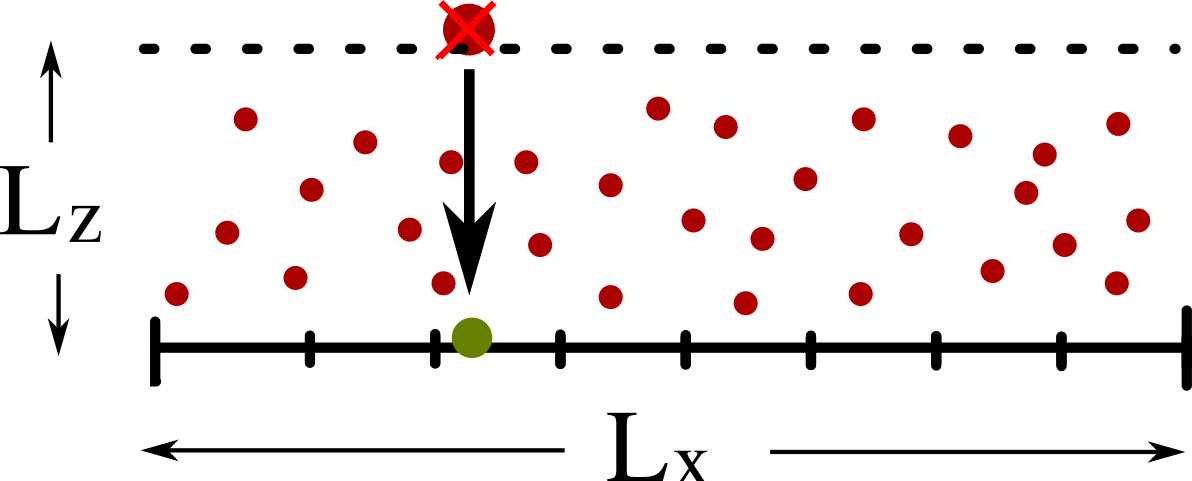
\includegraphics[width=\defaultwidth]{Fake_1d_3}
        \caption{Illustration of the noiseless convection model}
        \label{fig-fakez3}
      \end{figure}
      
      We have implemented this modified convection model in the \ac{2D} radial-azimuthal simulation.
      
      \Cref{fig-newconv_noconv} shows the time  evolution of the azimuthal electric field at the center of the radial dimension with and without the noiseless convection model.
      It presents the same conditions that in \cref{fig-convection_numerical}.{\bf a} and {\bf b}. 
      As previously, the convection stabilises the growth of the instability to a steady-state, but it does not affect the physics.
       
      
      \begin{figure}[hbtp]
        \centering
        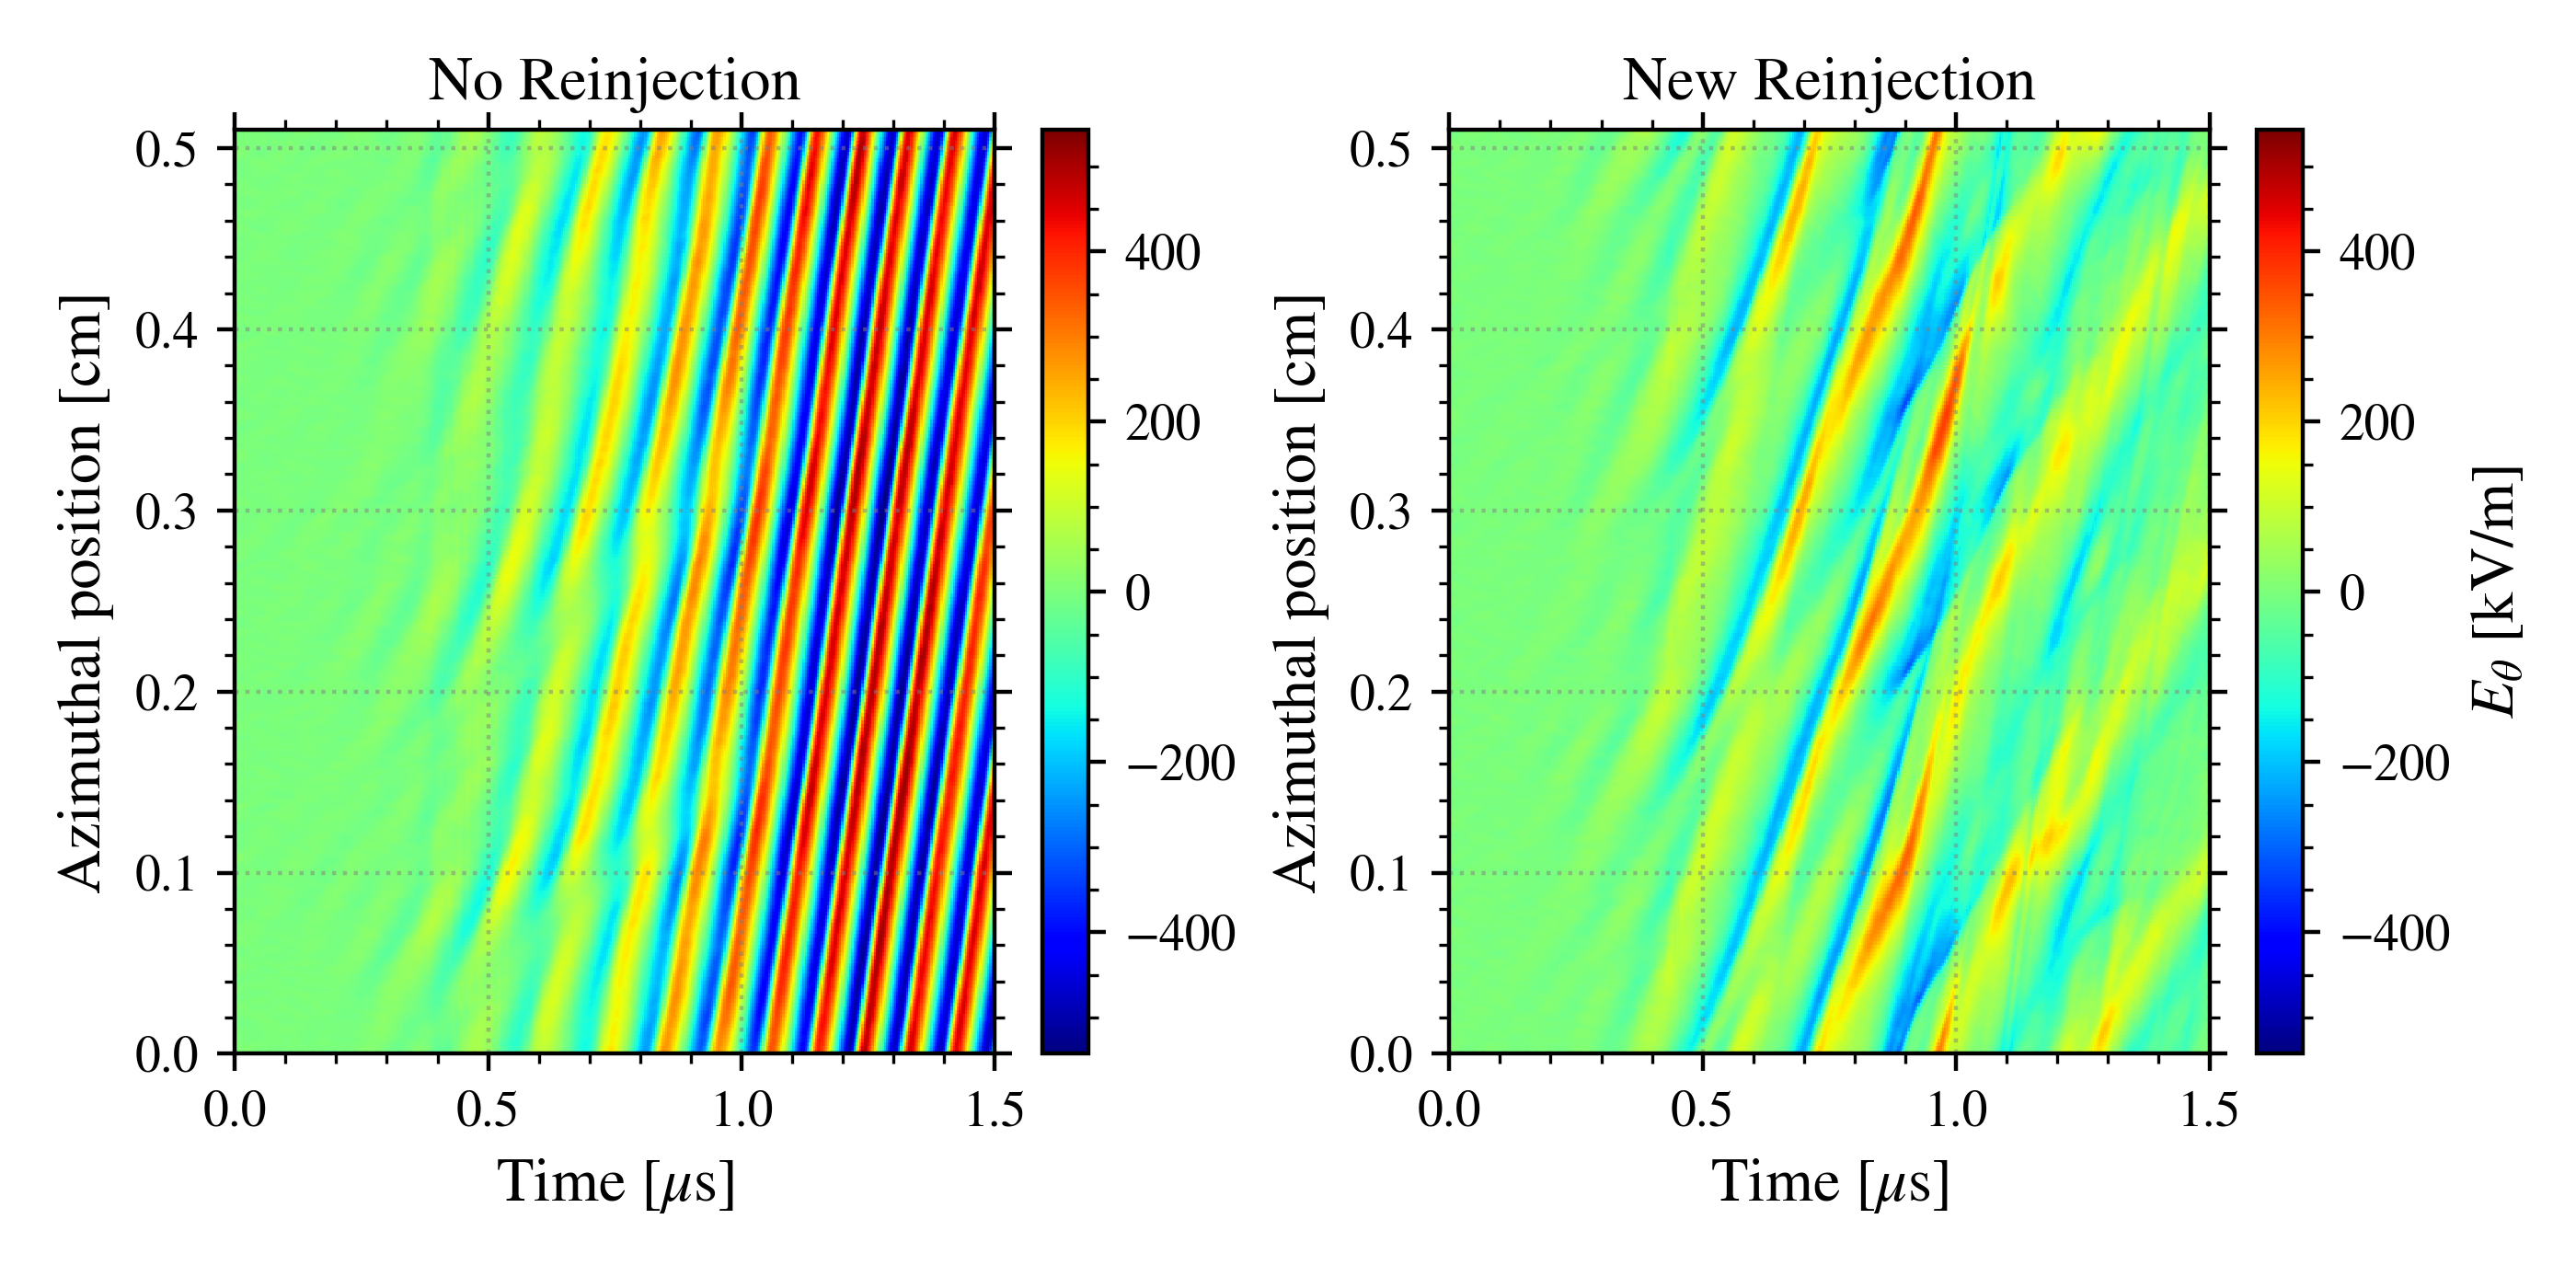
\includegraphics[width=\defaultwidth]{Compare_no_new_Reinj_Oz}
        \caption{Time evolution of the azimuthal electric field at the center of the radial dimension with and without the noiseless convection model. }
        \label{fig-newconv_noconv}
      \end{figure}
      
      \Cref{fig-oldeconv_newconv} shows the  time  evolution of the azimuthal electric field at the center of the radial dimension  with the convection modeled using Lafleur's model and the noiseless model with a small azimuthal length.
      We can see that the two models gives almost exactly the same results.
      
      \begin{figure}[hbtp]
        \centering
        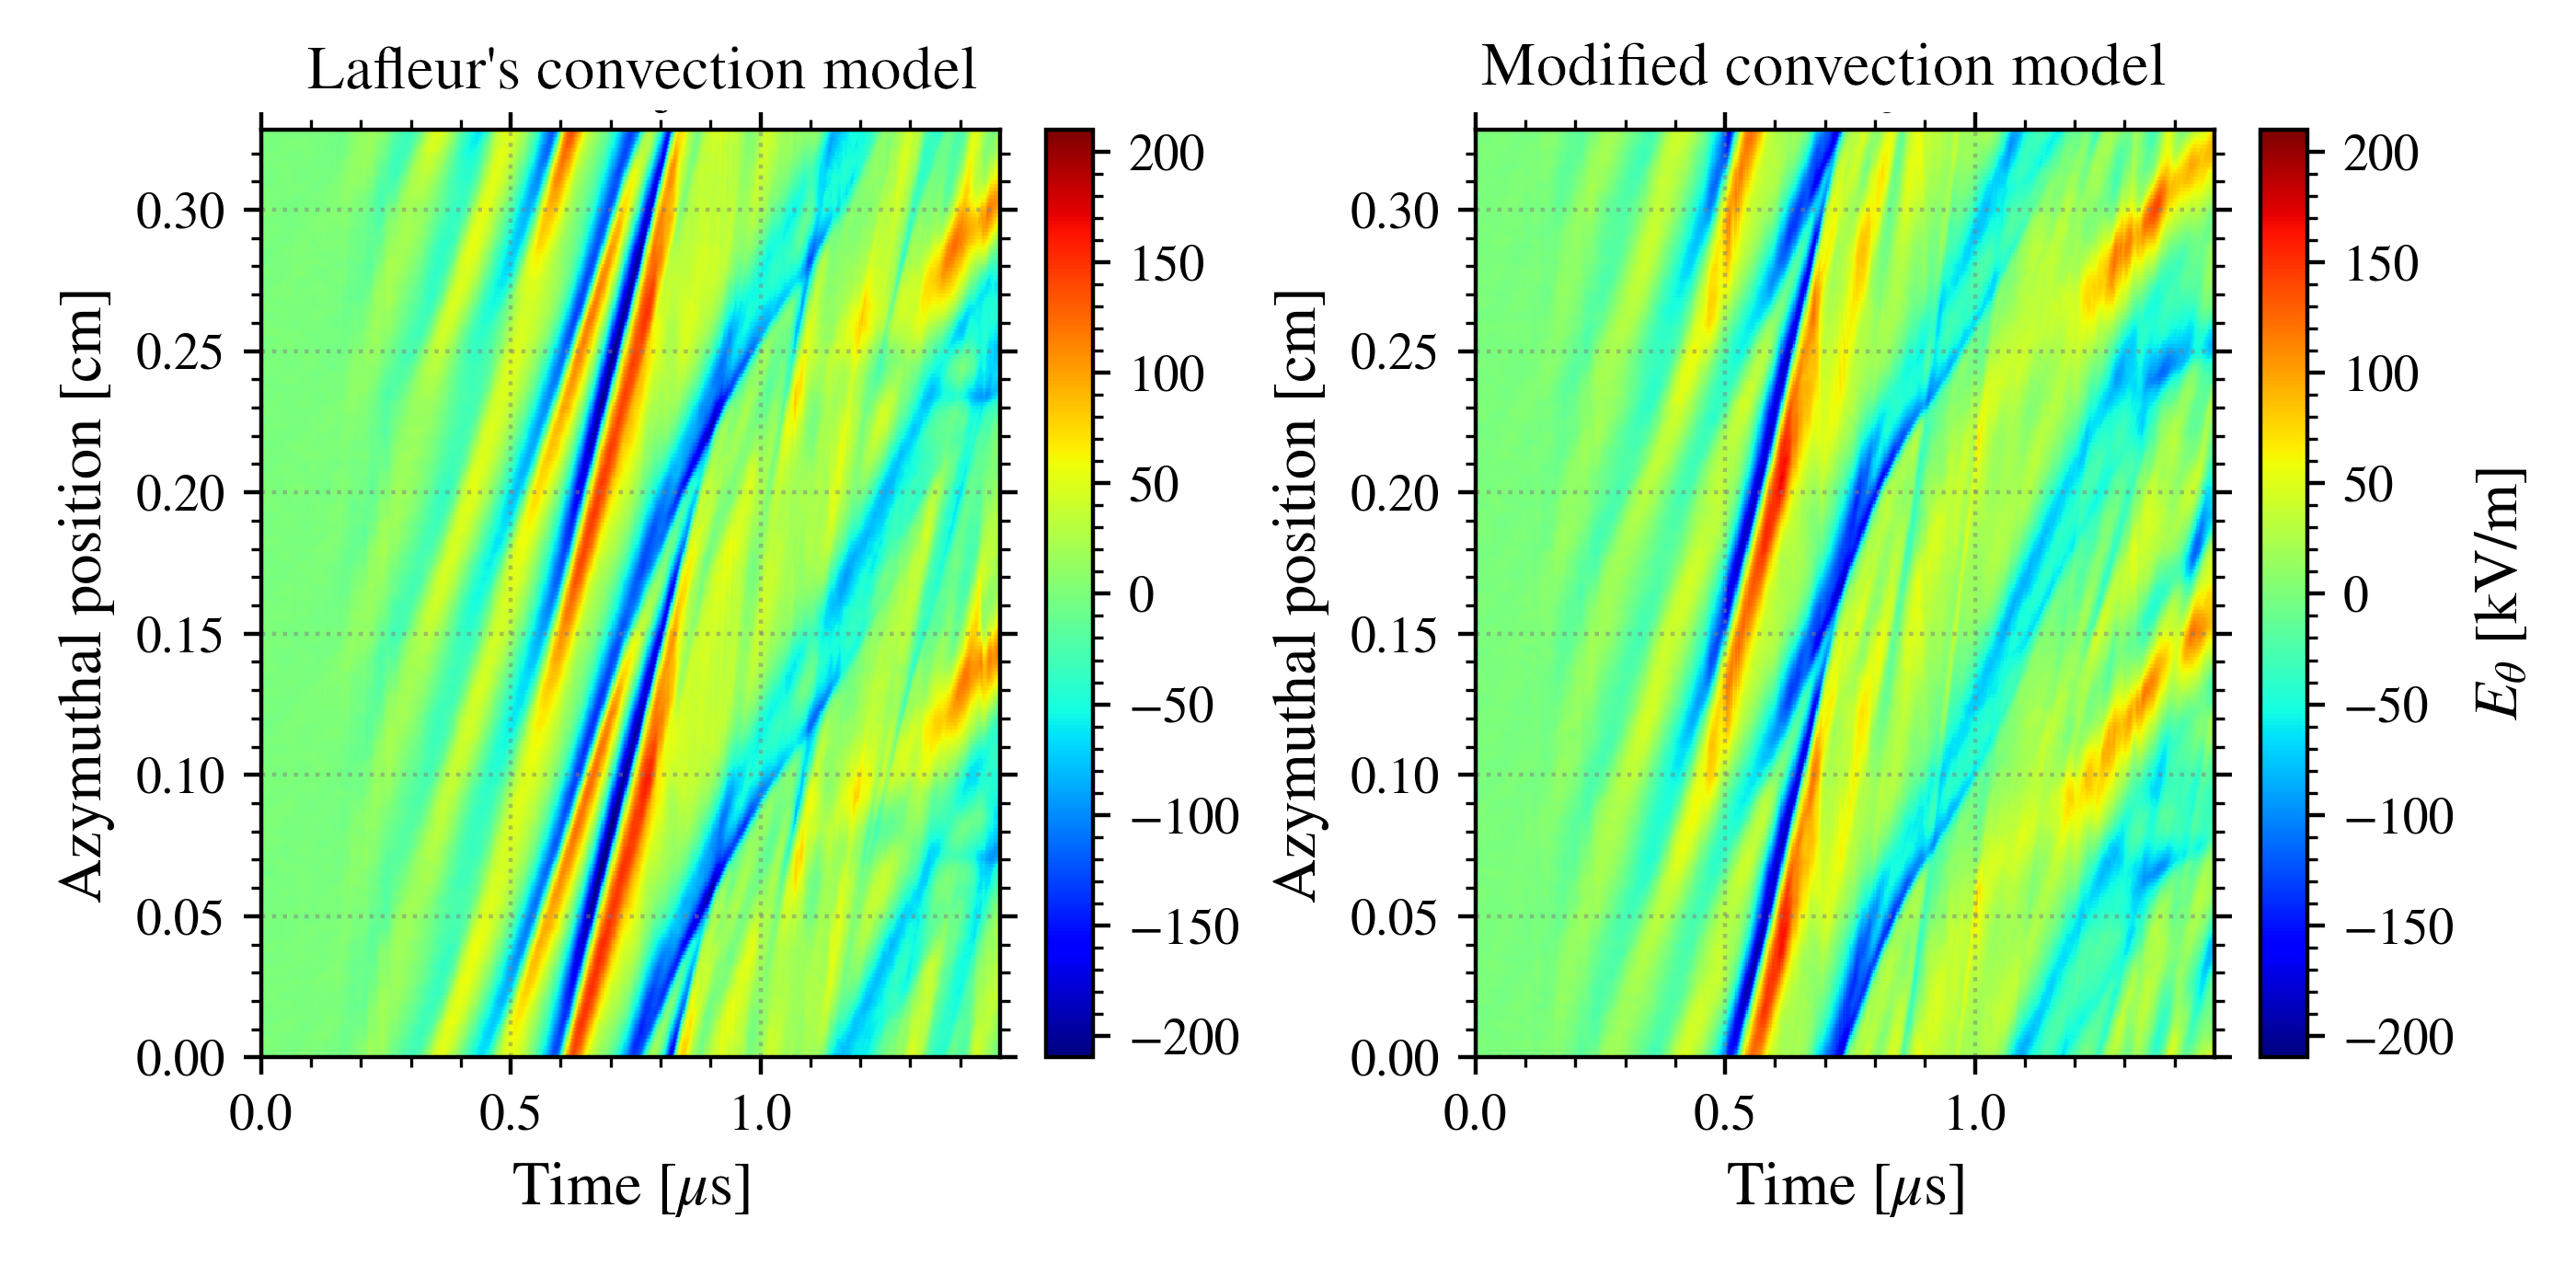
\includegraphics[width=\defaultwidth]{Compare_old_new_Reinj_Oz}
        \caption{Time evolution of the azimuthal electric field at the center of the radial dimension with the convection modeled using (left) Lafleur's model and (right) the noiseless model with a small azimuthal length.}
        \label{fig-oldeconv_newconv}
      \end{figure}
      
      
      \Cref{fig-oldeconv_newconv_longLZ} shows the  time  evolution of the azimuthal electric field at the center of the radial dimension  with the convection modeled using Lafleur's model and the noiseless model but using a longer azimuthal length than \cref{fig-oldeconv_newconv}.
      In this cases, we can see that Lafleur's convection model induces oscillations that are not observed with the noiseless model.
      
      \begin{figure}[hbtp]
        \centering
        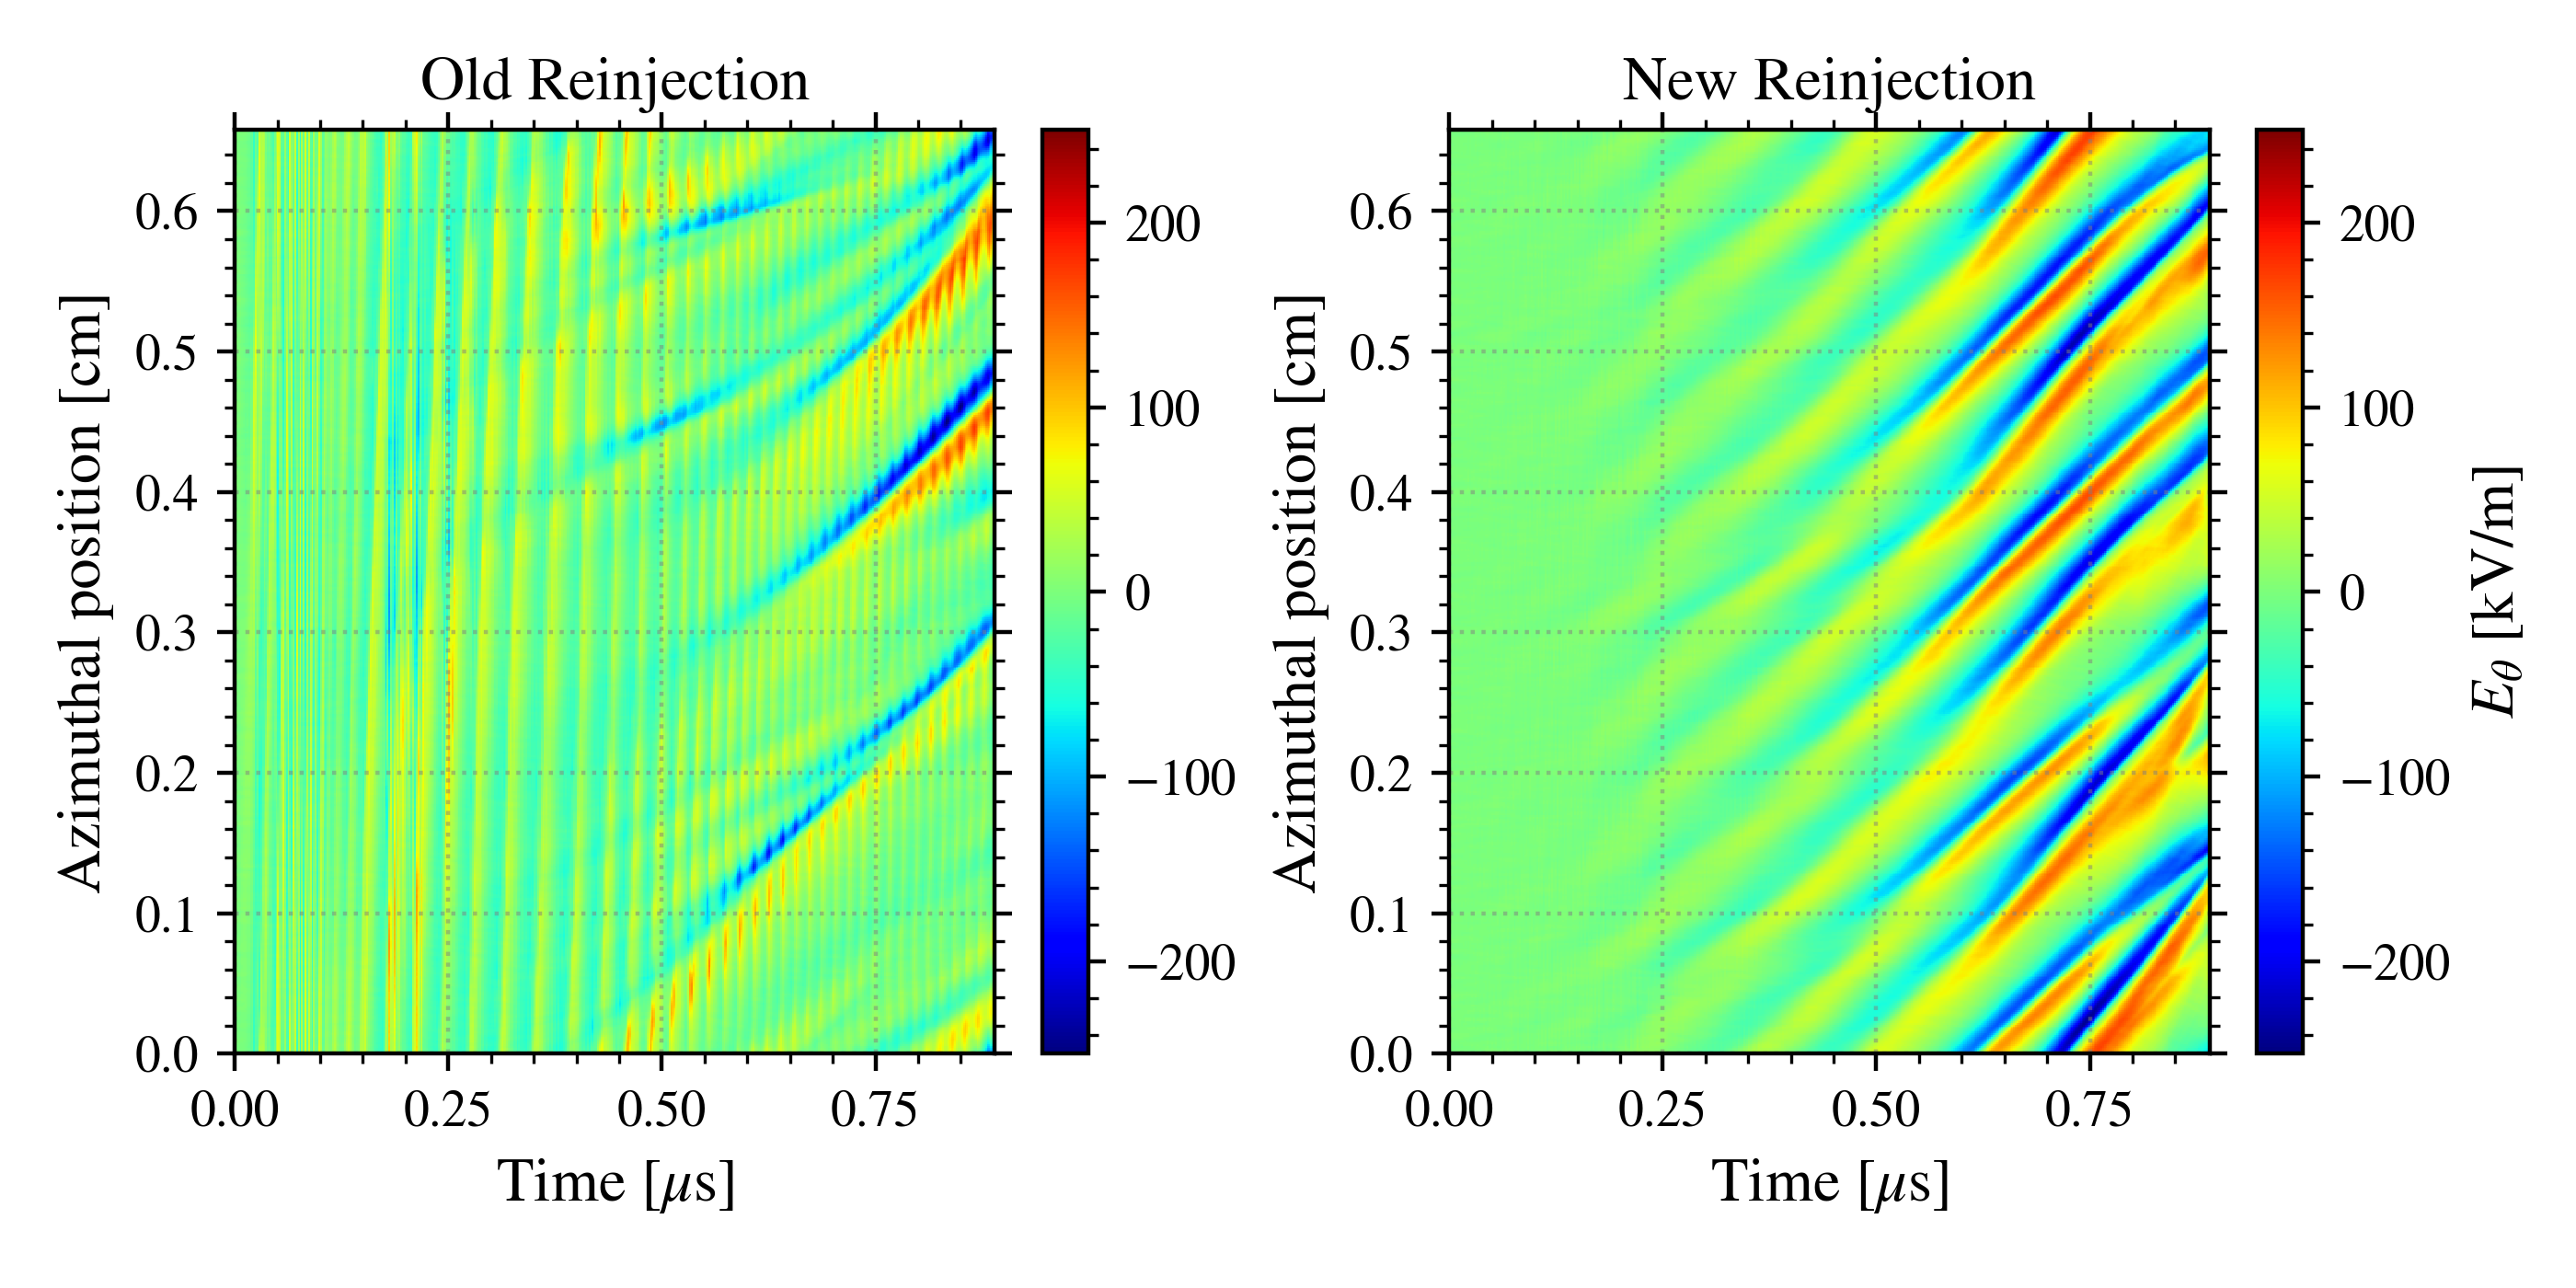
\includegraphics[width=\defaultwidth]{Compare_old_new_Reinj_Oz_LongLx}
        \caption{Time evolution of the azimuthal electric field at the center of the radial dimension with the convection modeled using (left) Lafleur's model and (right) the noiseless model with a longer azimuthal length.}
        \label{fig-oldeconv_newconv_longLZ}
      \end{figure}
      


      Theses observations hove shown that Trevor's convection model induces a noise on the charge density, that do not affect the simulation when the domain size is small, but can rise numerical artefacts when the domain size is larger.
      We have seen that the minor modification on the model do not affect the simulations results on a small domain, but allow us to use larger simulation domain without any numerical artefacts.
      
      \inlinenote{ Should we re-run all of the simulations of the 1rst paper using the new model ? Else, we should say why.}
    
    \subsection{Effects On a \ac{2D} simulation domain}
      
      The mathematical development of \cref{sec-mathnoise} has been done in \ac{1D}.
      We can legitimately ask is the results can be extended to a \ac{2D} domain.
      
      A mathematical definition of $\aziE_{, 1}$ is more difficult, as, neglecting the dielectric layers,
      \begin{equation} \label{eq-aziE}
        \aziE_{, 1} = \partial_{\theta} \phi_1 \text{ such that } \grad \cdot \grad \phi_1 = - \frac { \N(0, \stdconv)}{\epsilon_0} \text{ following the boundary condition}.
      \end{equation}
      
      However, we can investigate it numerically.
      \Cref{fig-dftLr} shows the \ac{DFT} of the source term $\rho_1 = \N(0, \stdconv)$, the resulting azimuthal electric field $\aziE_{, 1}$ and plasma potential $\rho$ computed on the centreline of the simulation domain in the radial direction, for three different radial length expressed in number of cell $N_x$.
      Is also discipled the "equivalent" source term $\rho_{\rm eq}$, which is the source term that would give the frequency spectra observed in a \ac{1D} domain
      \begin{equation} \label{eq-equirho}
        \rho_{\rm eq} = \partial_\theta \aziE_{, 1}.
      \end{equation}
      
      Using a Monte Carlo approach, the spectra are average over 50 cases in order to better observe the mean values of the distribution in respect with the standard deviation.
      
      \begin{figure}[hbtp]
        \centering
        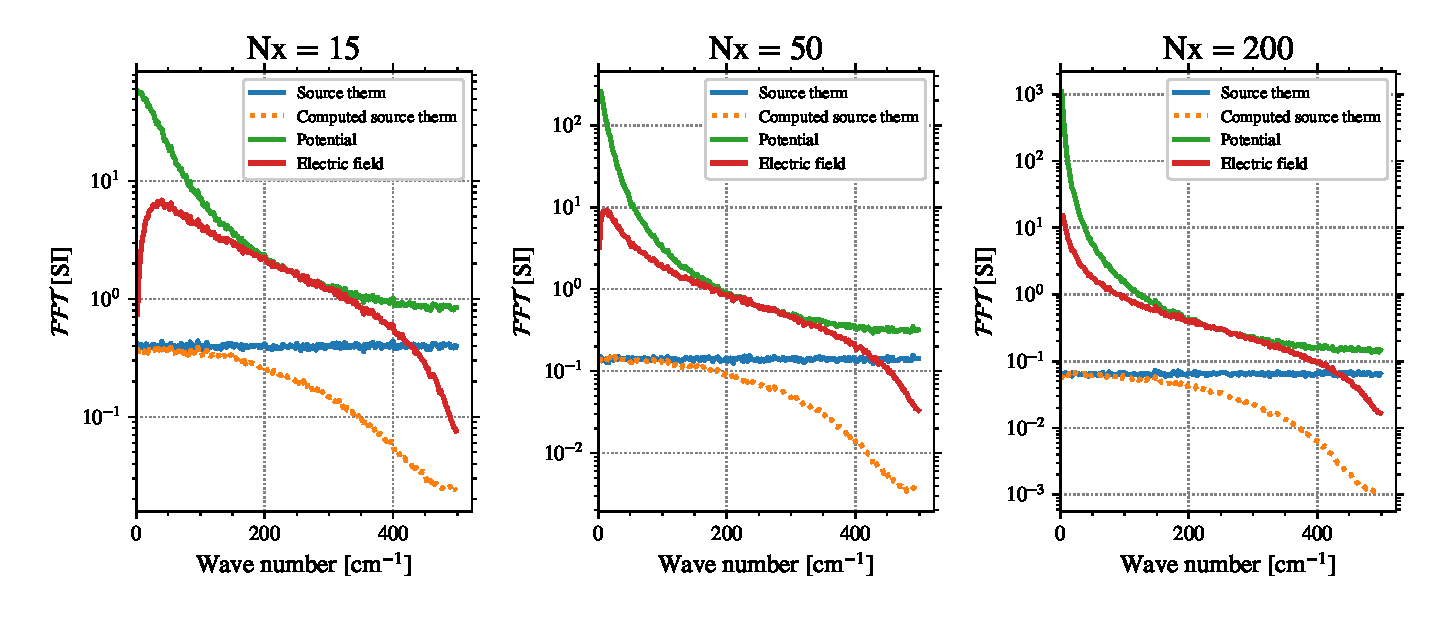
\includegraphics[width=\textwidth]{effect_Lr}
        \caption{\ac{DFT} of the source term $\rho_1 = \N(0, \stdconv)$, the resulting azimuthal electric field $\aziE_{, 1}$ and plasma potential $\rho$ computed on the centreline of a radial-azimuthal simulation. }
        \label{fig-dftLr}
      \end{figure}
      





